\newpage
\section*{BUILT-IN SYSTEM LOGGING}

The application needs to provide the ability of logging certain events or actions by using the built in system logging of a platform. 

\begin{center}
\ding{118} \ding{118} \ding{118}
\end{center}

\textbf{Having a variety of logging formats and log-file locations makes it hard to monitor the state of a whole enterprise, including all running applications.}\\

\textit{Format Variety.} A high variety of logging formats increases the complexity of integrating the information held within those several log files. It becomes a burden to nullify the different lay-outs of these log files.\\ 

\textit{Location Variety.} When having a variety of log file locations the dispersion of those locations makes it difficult to gather those files to one stack.\\

\textit{Information Granularity.} Not only the formats might be varying, but also the granularity of information. This makes it hard to monitor all applications in a consistent way or to integrate the information in a consistent way for other statistical purposes like e.g. root cause analysis\footnote{\url{http://en.wikipedia.org/wiki/Root_cause_analysis}}.

\begin{center}
\ding{118} \ding{118} \ding{118} 
\end{center}

\textbf{Therefore: Use the built-in system logging mechanism whenever possible. If it is not possible, then define a standard format to be used by all systems and implement your own logger.}\\

Many monitoring tools use the system built-in logging mechanisms. The connection between these is well defined and proven. It is therefore of help for the system administrators if these built-in logging mechanisms are used by all applications, as this allows the administrators to make use of existing tools (e.g. Nagios\footnote{\url{http://www.nagios.org/}} or HP OpenView) that collect, centralize, and search the logs \cite{Limoncelli2011a}.

The built-in system logging mechanisms take care of the log file location problem. They also prescribe the format, thereby forcing the developers, but also supporting them, to make consistent use of logging on the appropriate granularity.

It is also a lot easier to automatically generate incidents from specific defined events from the built-in system log for an IT service management (ITSM) tool. This ITSM tool can be configured to forward the automatically generated incidents directly, without human intervention, to the second line specialists. This way incidents are more easily solved without less human intervention, saving valuable time of the system administrators.

Of course logging in many cases has to be activated from within the system, so developers often have to explicitly program it into the system. But using the built-in logging mechanism alone does not ensure that the developers also make use of logging when it is appropriate. To address this issue guidelines could be defined and used by the developers for including logging in the system. 

If it is not possible to use the built-in system logging, e.g. because of different operating systems being used, then develop your own {\sc Diagnostic Logger} \cite{Harrison2001} and define a standard for your system landscape that works good in combination with the administration tools being used. Use the properties of built-in system logging mechanisms as basis for the requirements of your own logging mechanism. The most important point hereby is that this mechanism can be connected to the ITSM tools used by the system administrators. Ensure that this standard system is used for logging. This approach can be combined with {\sc Single File Location}.

Some requirements a good log should met to be valuable are:
\begin{itemize}
	\item Log actions before they happen.
	\item Mind the file size if logs should be copied or archived.
	\item Split messages into different files depending on intended audience/way of using.
\end{itemize}


To Do: \\
For implementing a (system) logging facility one can make use of the  pattern {\sc Memento} \cite{Gamma95} which is ... Writing to a log entry is best done with the pattern {\sc Command} \cite{Gamma95} and the logger itself is best implemented with pattern {\sc Factory} \cite{Gamma95}, which creates Mementos for logged events.

Add: Figure(s)

%\begin{figure}[h]
%\centering
%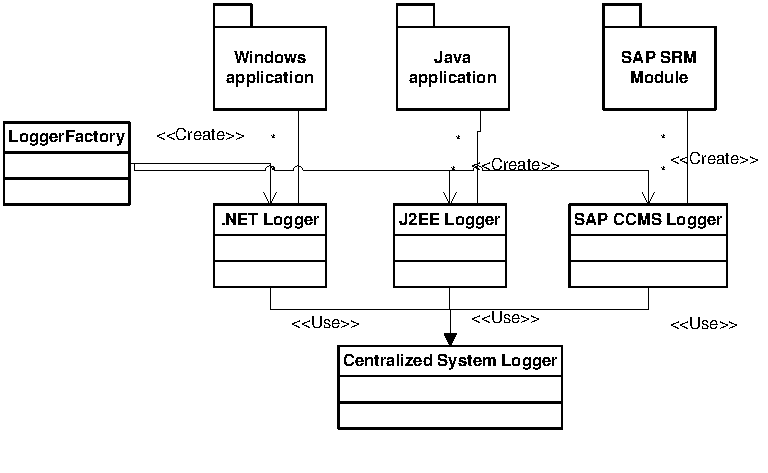
\includegraphics{patterns/systemLoggingDiagram.pdf}
%\caption{Main solution structure of BUILT-IN SYSTEM LOGGING}
%\label{fig:systemLogging}
%\end{figure}
%
%See figure \ref{fig:systemLogging}.

%\begin{center}
%\ding{118} \ding{118} \ding{118} 
%\end{center}





